%%%%%%%%%%%%%%%%%%%%%%%%%%%%%%%%%%%%%%%%%%%%%%%%%%%%%%%%%%%%%%%%%%%%%%%%%%%%%%%%%%
\begin{frame}[fragile]\frametitle{}

\begin{center}
{\Large Machine Learning in NLTK}
\end{center}
\end{frame}

%%%%%%%%%%%%%%%%%%%%%%%%%%%%%%%%%%%%%%%%%%%%%%%%%%%%%%%%%%%%%%%%%%%%%%%%%%%%%%%%%%
\begin{frame}[fragile]
\frametitle{Document classification NLTK example}
\begin{center}
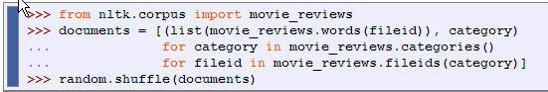
\includegraphics[width=\linewidth,keepaspectratio]{class8}
\end{center}
Define a feature extractor: a feature for each word, indicating whether the document contains that word. 
% \begin{center}
% 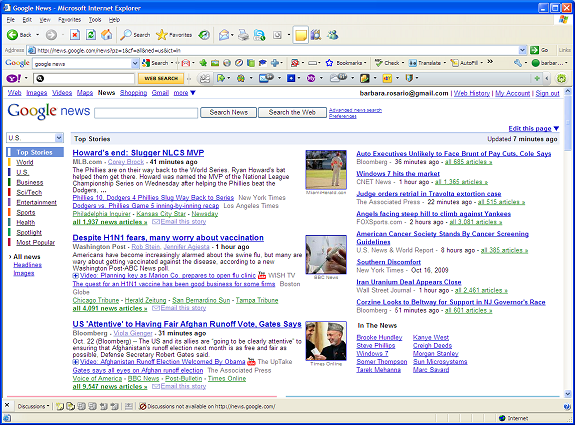
\includegraphics[width=\linewidth,keepaspectratio]{class9}
% \end{center}
\end{frame}

%%%%%%%%%%%%%%%%%%%%%%%%%%%%%%%%%%%%%%%%%%%%%%%%%%%%%%%%%%%%%%%%%%%%%%%%%%%%%%%%%%
\begin{frame}[fragile]
\frametitle{Document classification NLTK example}
Now that we've defined our feature extractor, we can use it to train a classifier
\begin{center}
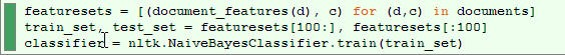
\includegraphics[width=\linewidth,keepaspectratio]{class10}
\end{center}
To check how reliable the resulting classifier is, we compute its accuracy on the test set 

\begin{center}
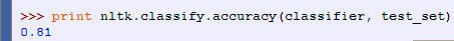
\includegraphics[width=\linewidth,keepaspectratio]{class11}
\end{center}
\end{frame}

%%%%%%%%%%%%%%%%%%%%%%%%%%%%%%%%%%%%%%%%%%%%%%%%%%%%%%%%%%%%%%%%%%%%%%%%%%%%%%%%%%
\begin{frame}[fragile]
\frametitle{Document classification NLTK example}
We can examine the classifier to determine which features it found most effective for distinguishing the review’s sentiment 

\begin{center}
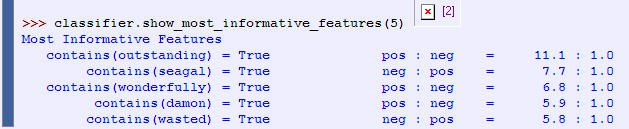
\includegraphics[width=\linewidth,keepaspectratio]{class12}
\end{center}
Apparently in this corpus, a review that mentions "Seagal" is almost 8 times more likely to be negative than positive, while a review that mentions "Damon" is about 6 times more likely to be positive.


\end{frame}


